\Chapter{Tervezés}

\Section{Bevezetés}

A specifikációk alapján a programban a felhasználónak kell tudnia csomópontokat hozzáadni, szerkeszteni, és azokat összekötni más csomópontokkal. Továbbá az éppen aktuális munkáját a gráf szerkesztőn el kell tudni menteni, és a program újraindításánál visszatölteni azt. Ez utóbbi megvalósításához szükség van valamilyen "tárolóra", vagyis egy szerverre és egy adatbázisra. Ennél a fejezetnél már nem csak a látható programrészen van a hangsúly, hanem legalább ugyanakkora figyelmet kap a szerver oldal is az adatbázissal, hiszen azok is kiemelkedő részei az alkalmazásnak.

\Section{Technológia és architektúra a szerver oldalon}

Ahhoz, hogy a bevezetőben említett specifikációt megvalósító szoftvert meg tudjuk írni, először kijelöljük a megfelelő technológiákat és az architektúrát. A kliens-szerver architektúra megfelelő erre az alkalmazásra. A kliens egy böngészős frontend, ami egy API-n keresztül tud kommunikálni a backend szerverrel, amely perzisztensen tárolja az adatokat egy relációs adatbázisban. A kliens esetünkben a böngészőben futó \textbf{JavaScript} alkalmazás, míg a szerver egy \textbf{Python} nyelven íródott \textbf{Falcon API}-t használ, valamint \textbf{SQLite} adatbázist a tárolásra.
 
Hogy ez működjön a számítógépünkön, először telepíteni kell a \textbf{Python}-t, és a \textbf{pip}-et. A Python-t egyszerűen le lehet tölteni a hivatalos honlapról\cite{pyt}. Windows felhasználóként a Windowshoz készült 64-bites setup segítségével telepítettem fel az alkalmazást. A \ref{fig:pyt1} ábrán látható, hogy a Python telepítésével egyidejűleg lehetőségünk van a pip telepítésére is, ehhez azonban manuális telepítés szükséges.

\begin{figure}[h]
\centering
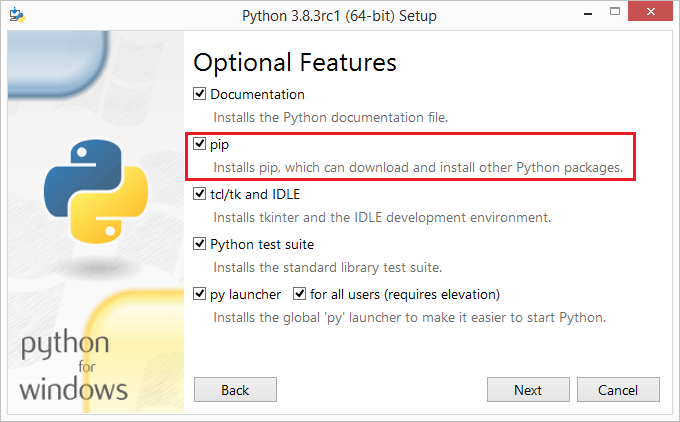
\includegraphics[scale=0.7]{images/python1.png}
\caption{Python telepítése pip-pel együtt}
\label{fig:pyt1}
\end{figure}

A telepítés következő lépésében célszerű bepipálni a 4. pontot, ami a környezeti változókhoz hozzáadja a Python-t (\texttt{Add Python to environment variables}), hiszen ennek elmulasztása esetén láthatósági problémák jelentkezhetnek használat közben.
%Lásd: \ref{fig:pyt2} ábra.

%\begin{figure}[h]
%\centering
%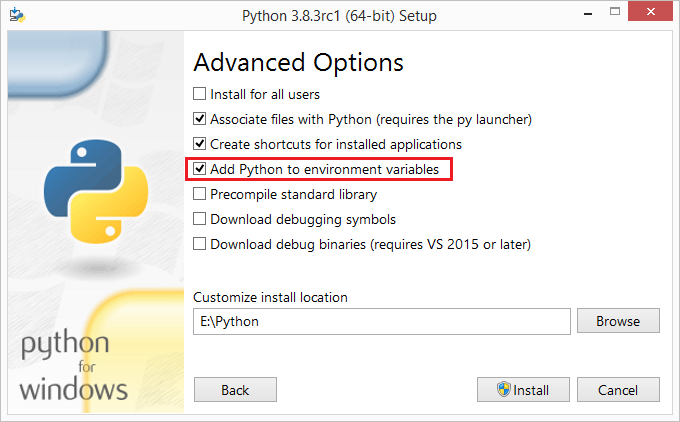
\includegraphics[scale=0.7]{images/python2.png}
%\caption{Python hozzáadása környezeti változókhoz}
%\label{fig:pyt2}
%\end{figure}

Ezek után a program működéséhez elengedhetetlen csomagokat telepítjük: az \textbf{SQLAlchemy}-t és a korábban említett \textbf{Falcon}-t. A telepítés a következő formátum megadásával történik: \texttt{python -m pip install [csomag neve]}

Tehát például a Falcon-t az alábbi parancs kiadása telepíti:

\begin{python}
python -m pip install falcon
\end{python}

Az SQLAlchemy-t pedig így a következő paranccsal fogjuk tudni telepíteni:
\begin{python}
python -m pip install sqlalchemy
\end{python}

Az SQLite3-at is érdemes telepítenünk, ha manuálisan akarjuk létrehozni az adatbázist és a táblákat. A telepítést itt is a hivatalos SQLite oldalon\cite{sqlite} keresztül tehetjük meg.

Ezt követően egy webszerver telepítése következik, például \textbf{waitress} vagy Unix-szerű rendszerek esetében a \textbf{gunicorn}, amivel elérhetjük a programot egy porton keresztül. Esetünkben a 8000-es portot használjuk. A backend szerver egy API-n keresztül szolgálja fel a statikus elemeket is, mint a HTML, CSS, JavaScript fájlokat.
 
Itt láthatjuk az útvonalakat, amelyeken az API felszolgálja a statikus elemeket:

\begin{python}
api.add_route('/js/{filename}', StaticJS())
api.add_route('/css/{filename}', StaticCSS())
api.add_route('/{filename}', StaticHTML())
\end{python}

A backend programban a Falcon keretrendszer kezeli az API-t, és egy adatbázis-kezelő segítségével csatlakozunk az adatbázishoz az alábbi módon:

\begin{python}
api = falcon.API()
dbms = mydatabase.MyDatabase(mydatabase.SQLITE, username='', password='', 
dbname='mydb.sqlite')
\end{python}

Az adatbázis-kezelő osztály tartalmaz metódusokat, amikkel az alapvető műveleteket elvégezhetjük, mint például a lekérdezést, beszúrást, törlést.

\begin{python}
# beszuras, torles
    def execute_query(self, query=''):
            if query == '' : return
            print (query)
            with self.db_engine.connect() as connection:
                try:
                    connection.execute(query)
                except Exception as e:
                    print(e)
def get_all_data(self, table='', query=''):
            query = query if query != '' else "SELECT * 
FROM '{}';".format(table)
            print(query)
            returnData = []
            with self.db_engine.connect() as connection:
                try:
                    result = connection.execute(query)
                except Exception as e:
                    print(e)
                else:   
                    for row in result:
                        print(row) # print(row[0], row[1], row[2])
                        d = dict(row.items())
                        returnData.append(d)
                    result.close()
            print("\n")       
            return returnData
\end{python}

A szerver egy REST API-n keresztül hallgat a kérésekre. Ezen az API-n szolgálja fel a statikus fájlokat, köztük a kliens programot is, és itt kommunikál a klienssel. Az \texttt{/api/nodes} végponton HTTP GET kéréssel felszolgáljuk az adatokat JSON formátumban az alábbi módon:
%Lásd: \ref{fig:get} ábra.

\begin{json}
[
   {
      "text":"folyamatElso",
      "height":50,
      "width":688,
      "radius":0,
      "y":540,
      "x":887,
      "type":"rectangle",
      "id":1
   },
   {
      "text":"folyamatMasodik",
      "height":50,
      "width":156,
      "radius":0,
      "y":512,
      "x":446,
      "type":"rectangle",
      "id":2
   },
   {
      "text":"",
      "height":0,
      "width":0,
      "radius":40,
      "y":122,
      "x":55,
      "type":"start",
      "id":3
   },
   {
      "text":"kezdo",
      "height":0,
      "width":0,
      "radius":40,
      "y":675,
      "x":1195,
      "type":"start",
      "id":4
   }
]
\end{json}

%\begin{figure}[h]
%\centering
%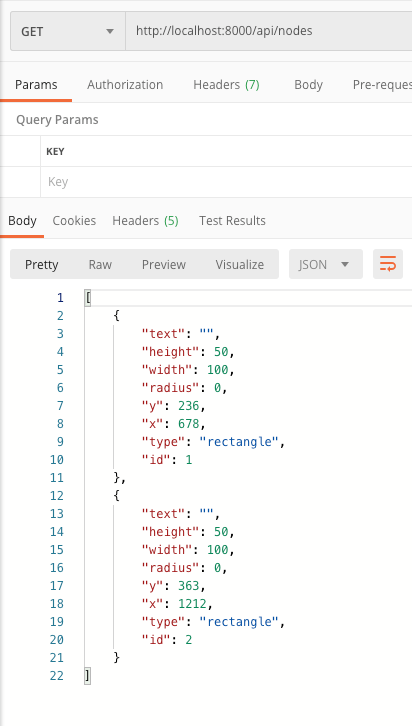
\includegraphics[scale=0.9]{images/get.png}
%\caption{GET kérés}
%\label{fig:get}
%\end{figure}

Ugyanezen a végponton HTTP POST kérés után mentjük az adatokat, amelynek a sikerességéről egy JSON válasz tájékoztat a következőképpen:
%Ez a \ref{fig:post} ábrán látható.

\begin{json}
[
   {
      "text":"",
      "height":50,
      "width":100,
      "radius":0,
      "y":236,
      "x":678,
      "type":"rectangle",
      "id":1
   },
   {
      "text":"",
      "height":50,
      "width":100,
      "radius":0,
      "y":363,
      "x":1212,
      "type":"rectangle",
      "id":2
   }
]
\end{json}

%\begin{figure}[h]
%\centering
%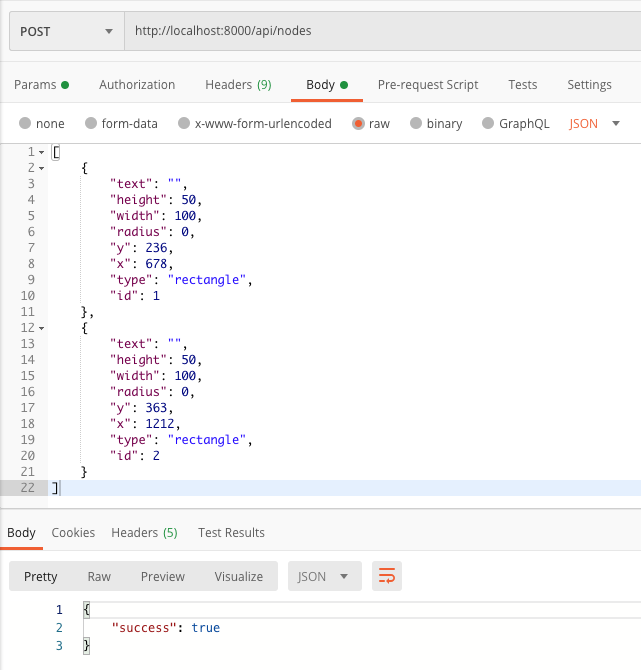
\includegraphics[scale=0.6]{images/post.png}
%\caption{POST kérés}
%\label{fig:post}
%\end{figure}

Az API azért REST, mert követi a REST architektúrát, azaz a web URL és kérés metódus által pontosan azonosítható, mit akar a kliens. Például ha a metódus GET és az URL \texttt{/api/nodes} az azt jelenti, hogy a kliens le szeretné kérni az összes csomópontot.
 
A szerver a már fentebb említett SQLite adatbázissal is kommunikál, itt perzisztensen tároljuk az adatokat, így a következő indításnál is megmarad minden a szerkesztőben.

Az adatbázis két táblát használ, a \textbf{nodes} és az \textbf{edges} táblákat. Először manuálisan kell létrehozni őket, az alábbi ER diagram szerint:

\begin{figure}[h]
\centering
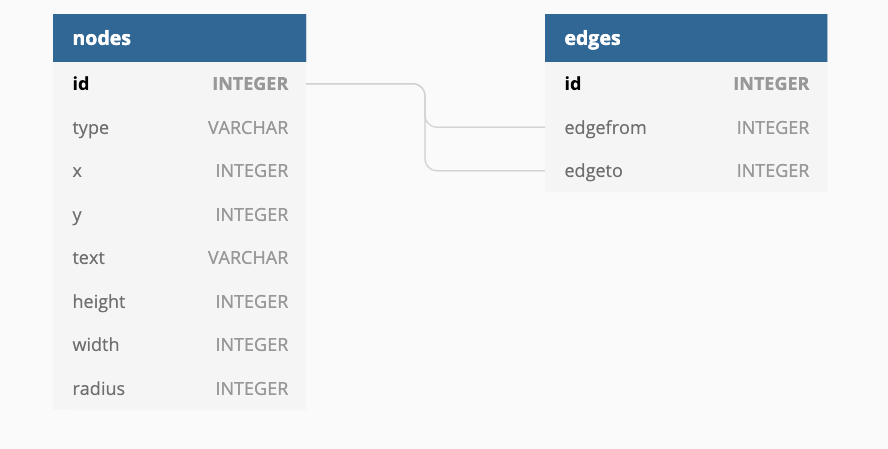
\includegraphics[scale=0.65]{images/sqltables.png}
\caption{SQL táblák ER diagramja}
\label{fig:sql}
\end{figure}

SQLAlchemy-ben így néz ki a fenti séma:

\begin{python}
            nodes = Table(NODES, metadata,
                        Column('id', Integer, primary_key=True),
                        Column('type', String),
                        Column('x', Integer),
                        Column('y', Integer),
                        Column('text', String),
                        Column('height', Integer),
                        Column('width', Integer),
                        Column('radius', Integer)
                        )
            edges = Table(EDGES, metadata,
                        Column('id', Integer, primary_key=True),
                        Column('edgefrom', Integer, 
ForeignKey("nodes.id"), nullable=False ),
                        Column('edgeto', Integer, 
ForeignKey("nodes.id"), nullable=False)
                        ) 
\end{python}

\newpage

\Section{A kliens oldal}
A JavaScript kliens program 9 osztályból áll. Az osztályok mind külön feladatot látnak el. Az \textbf{Editor} osztály körül öleli a többi osztályt, és megosztja közöttük az információkat. A \textbf{Graph} osztály kezeli a szerkesztőt. A szerkesztő és tartalma megrajzolása ebben az osztályban valósul meg. Minden, a szerkesztőn megjelenő elem, ennek az osztálynak valamelyik adattagjában megtalálható. Két fontos adattagja a \textbf{nodes} és \textbf{edges} tömbök, melyek a \textbf{Node} és \textbf{Edge} osztályok, vagy ezen osztályok egyik leszármazottjának a példányait tartalmazzák. A Node osztály tartalmazza a csomópontokat a különböző alakzataival, míg az Edge osztály az alakzatokat összekötő vonalakat valósítja meg.
 
A Node osztálynak 3 közvetlen leszármazottja van: \textbf{Diamond}, \textbf{Rectangle} és \textbf{Circle} (magyarul: rombusz, téglalap és kör) melyek mind implementálják a Node osztály konstruktorát. A Circle osztálynak további két leszármazottja van: a \textbf{Start} és az \textbf{End}, melyek a kezdő- és végállapotokat jelölik.

Ezen osztályoknak mind vannak saját metódusai, melyek ugyanazokat a funkciókat látják el, csak a részletekben térnek el. Ilyen például a \textit{resize()} és \textit{draw()} metódus. Mivel minden alakzatot meg kell rajzolni, vagy adott esetben átméretezni, ezek a metódusok minden alakzatot megvalósító osztályban megtalálhatóak, és a legtöbb funkció végrehajtásakor ezek meg is hívódnak.
 
A frontend egy API-n, \textbf{HTTP kérések}kel kommunikál a szerverrel. A mentés úgy zajlik, hogy a frontend alkalmazás összegyűjti az összes csomópontot és az őket összekötő vonalakat, majd egy objektumot csinál minden egyes csomópontból és vonalból csak a szükséges adatokkal, ezt követően pedig hozzáadja egy tömbhöz. Ezután JSON formátumba alakítja a tömbben lévő objektumokat, amit egy \textbf{HTTP POST} kéréssel elküldünk a szervernek.

A lekéréshez \textbf{HTTP GET} kérést használunk, itt JSON formátumú tömböt kapunk benne a megfelelő adatokat tartalmazó objektumokkal. Ezeket az adatokat visszaalakítjuk, hozzájutva így a megfelelő osztályok konstruktorainak paramétereihez. Ezután a paraméterekkel osztályt hozunk létre belőle, és ezeket az osztályokat hozzáadjuk a Graph osztály nodes és edges adattagjaihoz. Innentől kezdve tudjuk reprezentálni őket a kliens alkalmazással.